\documentclass{beamer}
\usetheme{Warsaw}

\usepackage{graphicx} % Allows including images
\usepackage{booktabs} % Allows the use of \toprule, \midrule and \bottomrule in tables
\usepackage{listings}
\usepackage[utf8]{inputenc}
\usepackage[overlay,absolute]{textpos}
\usepackage{tikz}
\usetikzlibrary{arrows, automata}

\AtBeginSection[]
{
\begin{frame}<beamer>
\frametitle{Plan}
\tableofcontents[
  currentsection,
  hideothersubsections
]
\end{frame}
}

\lstset{language=C++,
                basicstyle=\ttfamily,
                keywordstyle=\color{green}\ttfamily,
                stringstyle=\color{red}\ttfamily,
                commentstyle=\color{cyan}\ttfamily,
                morecomment=[l][\color{magenta}]{\#}
}

\setbeamercolor{normal text}{fg=white,bg=black!90}
\setbeamercolor{structure}{fg=white}

\setbeamercolor{alerted text}{fg=red!85!black}

\setbeamercolor{item projected}{use=item,fg=black,bg=item.fg!35}

\setbeamercolor*{palette primary}{use=structure,fg=structure.fg}
\setbeamercolor*{palette secondary}{use=structure,fg=structure.fg!95!black}
\setbeamercolor*{palette tertiary}{use=structure,fg=structure.fg!90!black}
\setbeamercolor*{palette quaternary}{use=structure,fg=structure.fg!95!black,bg=black!80}

\setbeamercolor*{framesubtitle}{fg=white}

\setbeamercolor*{block title}{parent=structure,bg=black!60}
\setbeamercolor*{block body}{fg=black,bg=black!10}
\setbeamercolor*{block title alerted}{parent=alerted text,bg=black!15}
\setbeamercolor*{block title example}{parent=example text,bg=black!15}

\author[Félix-Antoine Ouellet]{Félix-Antoine Ouellet}

\title[Sanitizer\hspace{2em}\insertframenumber/\inserttotalframenumber]{Détection dynamique de conditions de course}

\institute{Université de Sherbrooke}

\date{6 novembre 2014}

\begin{document}

\begin{frame}
\titlepage % Print the title page as the first slide
\end{frame}

\begin{frame}
\tableofcontents[hideallsubsections]
\end{frame}

\section{Motivation}
\begin{frame}
\frametitle{Condition de course}
\framesubtitle{Définition}
Situation se produisant quand 2 \textit{threads} accèdent à la même structure partagée sans contraintes d'ordonnancement et qu'un de ces accès est une écriture.
\end{frame}

\begin{frame}[fragile]
\frametitle{Condition de course}
\framesubtitle{Example - Trivial}
\begin{lstlisting}
int main() {
  int X = 0;
  std::thread T([&](){ X = 42; });
  X = 43;
  T.join();
}
\end{lstlisting}

Que vaut X à la fin du programme?
\end{frame}

\begin{frame}[fragile]
\frametitle{Condition de course}
\framesubtitle{Example - Moins trivial}
\begin{lstlisting}
Singleton* Singleton::getInstance() {
  if (m_Instance == nullptr) {
    std::lock_guard<std::mutex> Lock(m_Mutex);
    {
      if (m_Instance == nullptr) {
        m_Instance = new Singleton;      
      }
    }  
  }
  return m_Instance;
}
\end{lstlisting}
\end{frame}

\section{Arrivé-avant}
\subsection{Idée}
\begin{frame}
\frametitle{Idée}
Un programme parallèle sans condition de course ne comporte que des accès ordonnancés à des structures partagées
\end{frame}

\subsection{Concepts de base}
\begin{frame}
\frametitle{Opérations de synchronisation}
\framesubtitle{Théorie}
\begin{itemize}
\item Publication: Rend publique de l'information produite par le \textit{thread}
\item Réception: Lecture d'une information publique
\end{itemize}
\end{frame}

\begin{frame}
\frametitle{Opérations de synchronisation}
\framesubtitle{Pratique}
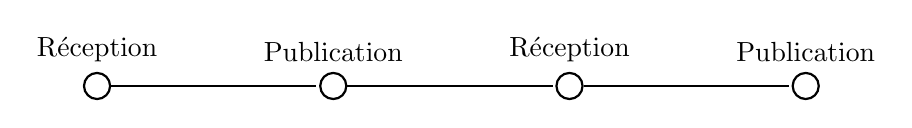
\begin{tikzpicture}[-,>=stealth',shorten >=1pt,auto,node distance=3cm,
  thick,main node/.style={circle,draw,font=\sffamily\Large\bfseries}]

  \node[main node] (1) [label={above:Réception}] {};
  \node[main node] (2) [right of=1, label={above:Publication}] {};
  \node[main node] (3) [right of=2, label={above:Réception}] {};
  \node[main node] (4) [right of=3, label={above:Publication}] {};

  \path[every node/.style={font=\sffamily\small}]
    (1) edge node [right] {} (2)
    (2) edge node [right] {} (3)
    (3) edge node [right] {} (4);
\end{tikzpicture}
\end{frame}

\begin{frame}
\frametitle{Segments}
\framesubtitle{Théorie}
Suite d'opérations effectuées par un \textit{thread} se terminant par une opération de synchronisation
\end{frame}

\begin{frame}
\frametitle{Segments}
\framesubtitle{Pratique}
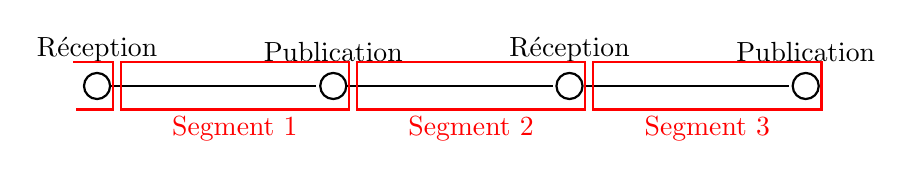
\begin{tikzpicture}[-,>=stealth',shorten >=1pt,auto,node distance=3cm,
  thick,main node/.style={circle,draw,font=\sffamily\Large\bfseries}]

  \node[main node] (1) [label={above:Réception}] {};
  \node[main node] (2) [right of=1, label={above:Publication}] {};
  \node[main node] (3) [right of=2, label={above:Réception}] {};
  \node[main node] (4) [right of=3, label={above:Publication}] {};

  \path[every node/.style={font=\sffamily\small}]
    (1) edge node [right] {} (2)
    (2) edge node [right] {} (3)
    (3) edge node [right] {} (4);
    
    \draw[red] (-0.3, 0.3) -- (0.2, 0.3) -- (0.2, -0.3) -- (-0.3, -0.3);
    \draw[red] (0.3, -0.3) rectangle (3.2, 0.3) node[pos=0.5, below, label={below:Segment 1}] {};
    \draw[red] (3.3, -0.3) rectangle (6.2, 0.3) node[pos=0.5, below, label={below:Segment 2}] {};
    \draw[red] (6.3, -0.3) rectangle (9.2, 0.3) node[pos=0.5, below, label={below:Segment 3}] {};
\end{tikzpicture}
\end{frame}

\begin{frame}
\frametitle{Ordonnancement des segments}
\framesubtitle{Théorie}
\begin{itemize}
\item Un ordre partiel peut être établi en fonction des opérations de synchronisation
\item Dénoté par l'opérateur $\prec$
\end{itemize}
\end{frame}

\begin{frame}
\frametitle{Ordonnancement des segments}
\framesubtitle{Pratique}
\begin{center}
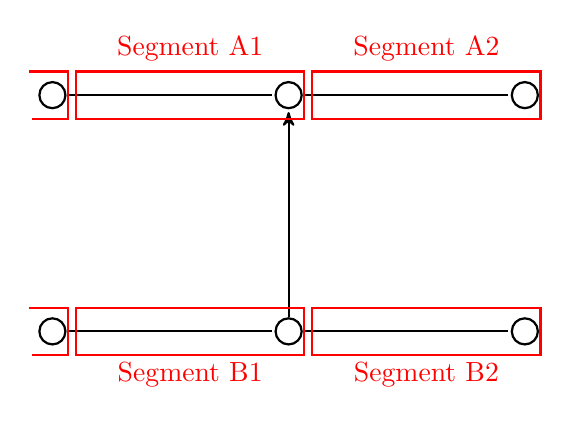
\begin{tikzpicture}[-,>=stealth',shorten >=1pt,auto,node distance=3cm,
  thick,main node/.style={circle,draw,font=\sffamily\Large\bfseries}]

  \node[main node] (1) [] {};
  \node[main node] (2) [right of=1] {};
  \node[main node] (3) [right of=2] {};
  \node[main node] (4) [below of=1] {};
  \node[main node] (5) [right of=5, below of=1] {};
  \node[main node] (6) [right of=6, below of=2] {};

  \path[every node/.style={font=\sffamily\small}]
    (1) edge node [right] {} (2)
    (2) edge node [right] {} (3)
    (4) edge node [right] {} (5)
    (5) edge node [right] {} (6);
    
  \path (5) edge [->] (2);  
  
  \draw[red] (-0.3, 0.3) -- (0.2, 0.3) -- (0.2, -0.3) -- (-0.3, -0.3);
  \draw[red] (0.3, -0.3) rectangle (3.2, 0.3) node[pos=0.5, below, label={[yshift=0.3cm]above:Segment A1}] {};  
  \draw[red] (3.3, -0.3) rectangle (6.2, 0.3) node[pos=0.5, below, label={[yshift=0.3cm]above:Segment A2}] {};
  
  \draw[red] (-0.3, -2.7) -- (0.2, -2.7) -- (0.2, -3.3) -- (-0.3, -3.3);
  \draw[red] (0.3, -3.3) rectangle (3.2, -2.7) node[pos=0.5, below, label={below:Segment B1}] {};  
  \draw[red] (3.3, -3.3) rectangle (6.2, -2.7) node[pos=0.5, below, label={below:Segment B2}] {};
\end{tikzpicture}
\end{center}

\only<2>{
\begin{textblock}{6}(1, 9)
	\textcolor{white}{Segment B1 $\prec$ Segment A2}
\end{textblock}
}
\end{frame}

\begin{frame}
\frametitle{Concepts de base}
\framesubtitle{Condition de course}

\end{frame}

\subsection{Algorithme}
\begin{frame}
\frametitle{Algorithme}

\end{frame}

\section{Ensemble de verrous}
\subsection{Idée}
\begin{frame}
\frametitle{Idée}
Un programme parallèle sans condition de course respecte toujours une saine discipline de verrouillage des structures partagées
\end{frame}

\subsection{Algorithme}
\begin{frame}
\frametitle{Algorithme}
\framesubtitle{Ébauche}
But: S'assurer que toute structure partagée soit protégée par un verrou
\end{frame}

\begin{frame}
\frametitle{Algorithme}
\framesubtitle{Ébauche}
Trois problèmes de l'algorithme précédent
\begin{itemize}
\item Initialisation
\item Structure seulement en lecture
\item Verrou lecture-écriture
\end{itemize}
\end{frame}

\begin{frame}
\frametitle{Algorithme}
\framesubtitle{Raffinement}
\begin{center}
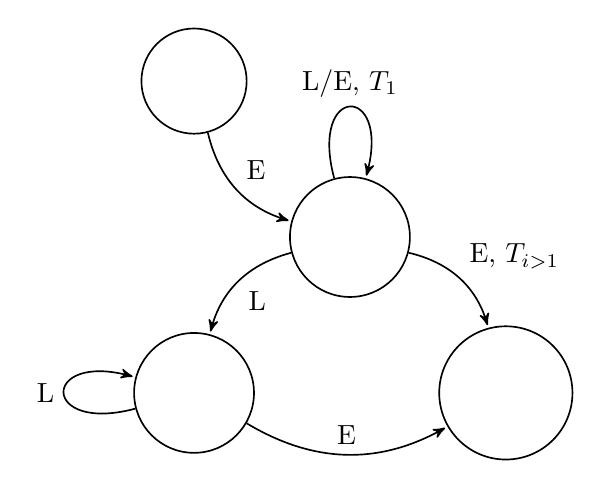
\begin{tikzpicture}[->,>=stealth',shorten >=1pt,auto,node distance=2.8cm,
                    semithick]
  \tikzstyle{every state}=[text=white]

  \node[state]         (A)                    {Exclusif};
  \node[state]         (B) [above left of=A] {Vierge};
  \node[state]         (D) [below left of=A] {Partagé};
  \node[state]         (C) [below right of=A, text width=1.2cm] {Partagé-Modifié};

  \path (A) edge [bend right] node {L} (D)
            edge [bend left]  node {E, $T_{i>1}$} (C)
            edge [loop above]  node {L/E, $T_{1}$} (A)
        (B) edge [bend right] node {E} (A)
        (D) edge [bend right] node {E} (C)
        (D) edge [loop left]  node {L} (B)
        ;
\end{tikzpicture}
\end{center}
\end{frame}

\begin{frame}
\frametitle{Algorithme}
\framesubtitle{Raffinement}

\begin{tikzpicture}[->,>=stealth',shorten >=1pt,auto,node distance=2.8cm,
                    semithick]
  \tikzstyle{every state}=[text=white]

  \node[state]         (A) [text width=1.2cm] {Partagé-Modifié};
\end{tikzpicture}

\begin{textblock}{5}(8, 7)
	 \textcolor{white}{TEST}
\end{textblock}
\end{frame}

\section{Conclusion}
\begin{frame}
\frametitle{Conclusion}
La plupart des outils de détection de condition de courses implémentent une variation ou une combinaison des algorithmes présentés.
\end{frame}

\end{document}